%%%%%%%%
% Highlevel
% ca 1-2 Seiten
% Buzzwords, grober Überriss
% Hier wird erklärt, mit welchem Ansatz an das Projekt herangegangen wurde
\section{Lösungsansatz}

% Warum wurde sich für die Darstellung der Mandelbrotmenge entschieden
\subsection{Verwendung der Mandelbrotmenge}

Es handelt bei der Bestimmung der Mandelbrotmenge um eine rechenintensive Operation, wobei
die benötigte Zeit durch Erhöhen der Iterationszahl beliebig erhöht werden kann.
Zusätzlich ist die Berechnung für jede einzelne komplexe Zahl unabhängig von
jeder anderen Zahl.

Diese Eigenschaften ermöglichen es zweierlei Dinge zu kontrollieren:
\begin{itemize}
	\item Die Dauer der Berechnung
	\item Die Aufteilung der Berechnung auf unterschiedliche Rechenkerne
\end{itemize}

Somit kann gesichert werden, dass eine wahrnehmbare Zeit (100-200 ms) zur Berechnung der Punkte innerhalb
der Mandelbrotmenge benötigt wird.
Aus didaktischer Sicht ist dies wichtig, um Differenzen zwischen den Balancierungsstrategien spürbar zu machen.
Zudem kann die Unterteilung des zu berechnden Raumes frei gewählt werden, sodass
verschiedenste Aufteilungen möglich sind und insbesondere bei der Lastbalancierung frei eingeteilt werden kann.

Als Projekt, das an nicht technisch versierten Anwendern spricht auch der ästethische
Faktor des Mandelbrotfraktals für eine Verwendung.
Er kann ein erstes Interesse für die Anwendung wecken.

% Wie ist die (grobe) Architektur des Programmes (parallelisiertes Backend, Oberfläche)
\subsection{Architekturübersicht}
\begin{figure}
	% Bindet das als PDF exportierte pptx ein -> vektorgrafik
	% -> pptx bearbeiten statt pdf
	\centering
	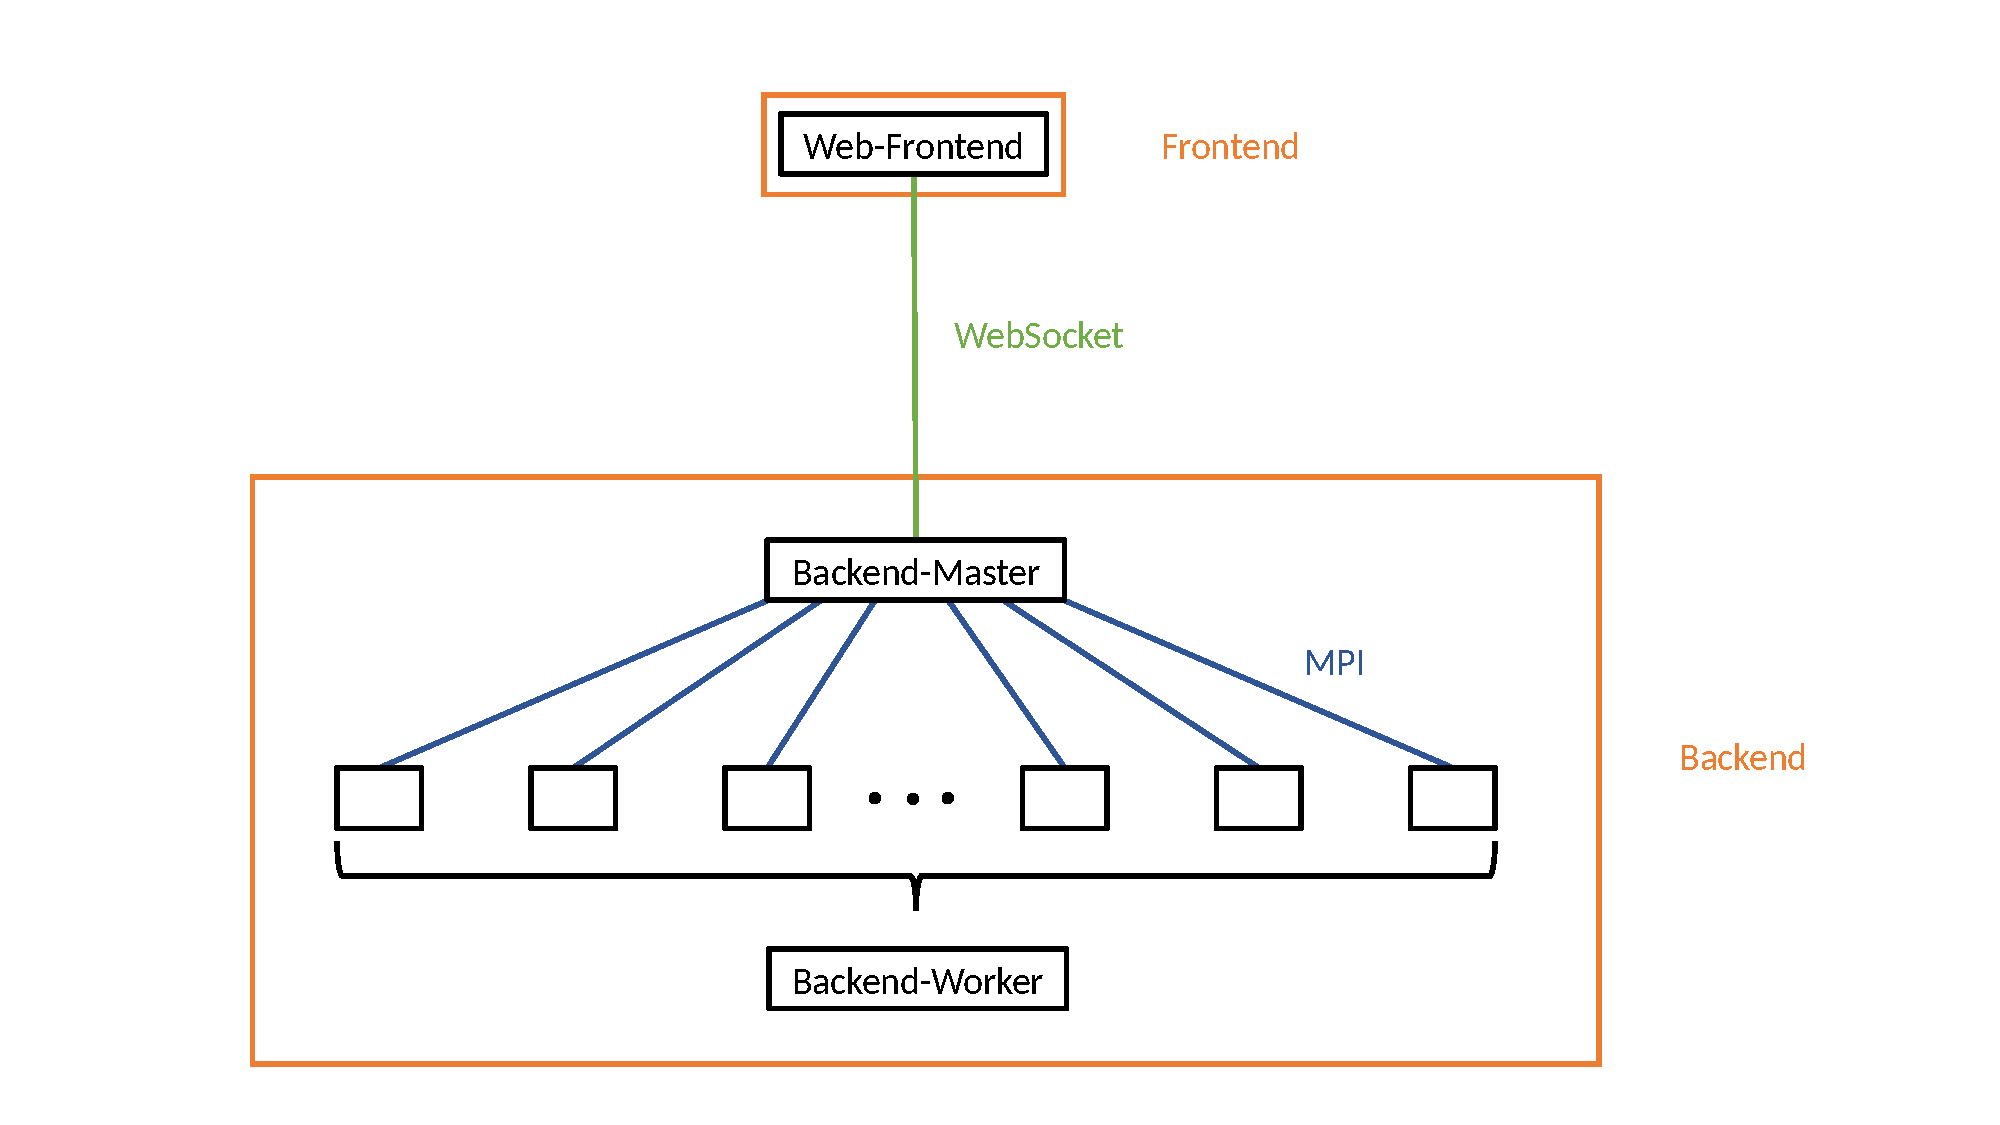
\includegraphics[width=0.98\linewidth]{img/Implementierung/Kommunikation.pdf}
	\caption{Architekturübersicht}
	\label{fig:architekturuebersicht}
\end{figure}

Die hohe Rechenintesivität sorgt dafür, dass der Berechnungsteil des Projektes möglichst in einer
hardwarenahen Sprache umgesetzt wird.
Andererseits sollte die Benutzeroberfläche einfach zu bedienen und auf möglichst vielen verschiedenen Geräten lauffähig sein.
Daher wurde sich für eine Unterteiltung in ein Frontend, im Browser aufrufbar, und ein Backend, auf einem Cluster
laufend und hardwarenah programmiert.

Zudem soll unterschieden werden, zwischen einem Host-Prozess im Backend, welcher für die Kommunikation mit dem
Frontend zuständig ist und Workerprozessen, welche die tatsächliche Berechnung der Mandelbrotmenge durchführen.
Der Hostprozess nimmt damit Rechenaufträge vom Nutzerfrontend entgegen und führt die Lastbalancierung durch.
Die kleineren Regionen der unterteilten Anfrage werden dann an die jeweiligen Workerprozesse gesendet, welche sie berechnen sollen.
Damit erhalten wir eine Unterteilung in drei wesentliche Bausteine, wie sie in \autoref{fig:architekturuebersicht} zu sehen sind.
\\ \\
ALTERNATIVE VERSION VOM TOBI KOMMT JETZT. HAB LEIDER NICHT GESEHEN, DAS DARAN SCHON WAS GEÄNDERT WURDE. WAS FINDET IHR BESSER?
\\ \\
\subsection{Architekturübersicht}
Die Architektur besteht aus drei wesentlichen Bausteinen, die in \autoref{fig:architekturuebersicht_detail} zu sehen sind:
\begin{itemize}
	\item Eine Benutzeroberfläche in einem Web-Browser (“Frontend”), die die Benutzerinteraktionen entgegennimmt und mit dem Backend kommuniziert.
	\item Ein Backend-Host, der eingehende Rechenaufträge vom Frontend an die Worker verteilt und deren Ergebnisse an das Frontend weiterleitet.
	\item Mehrere Backend-Worker, die die eigentliche Berechnung parallelisiert durchführen.
\end{itemize}
\begin{figure}[h!]
	% Bindet das als PDF exportierte pptx ein -> vektorgrafik
	% -> pptx bearbeiten statt pdf
	\centering
	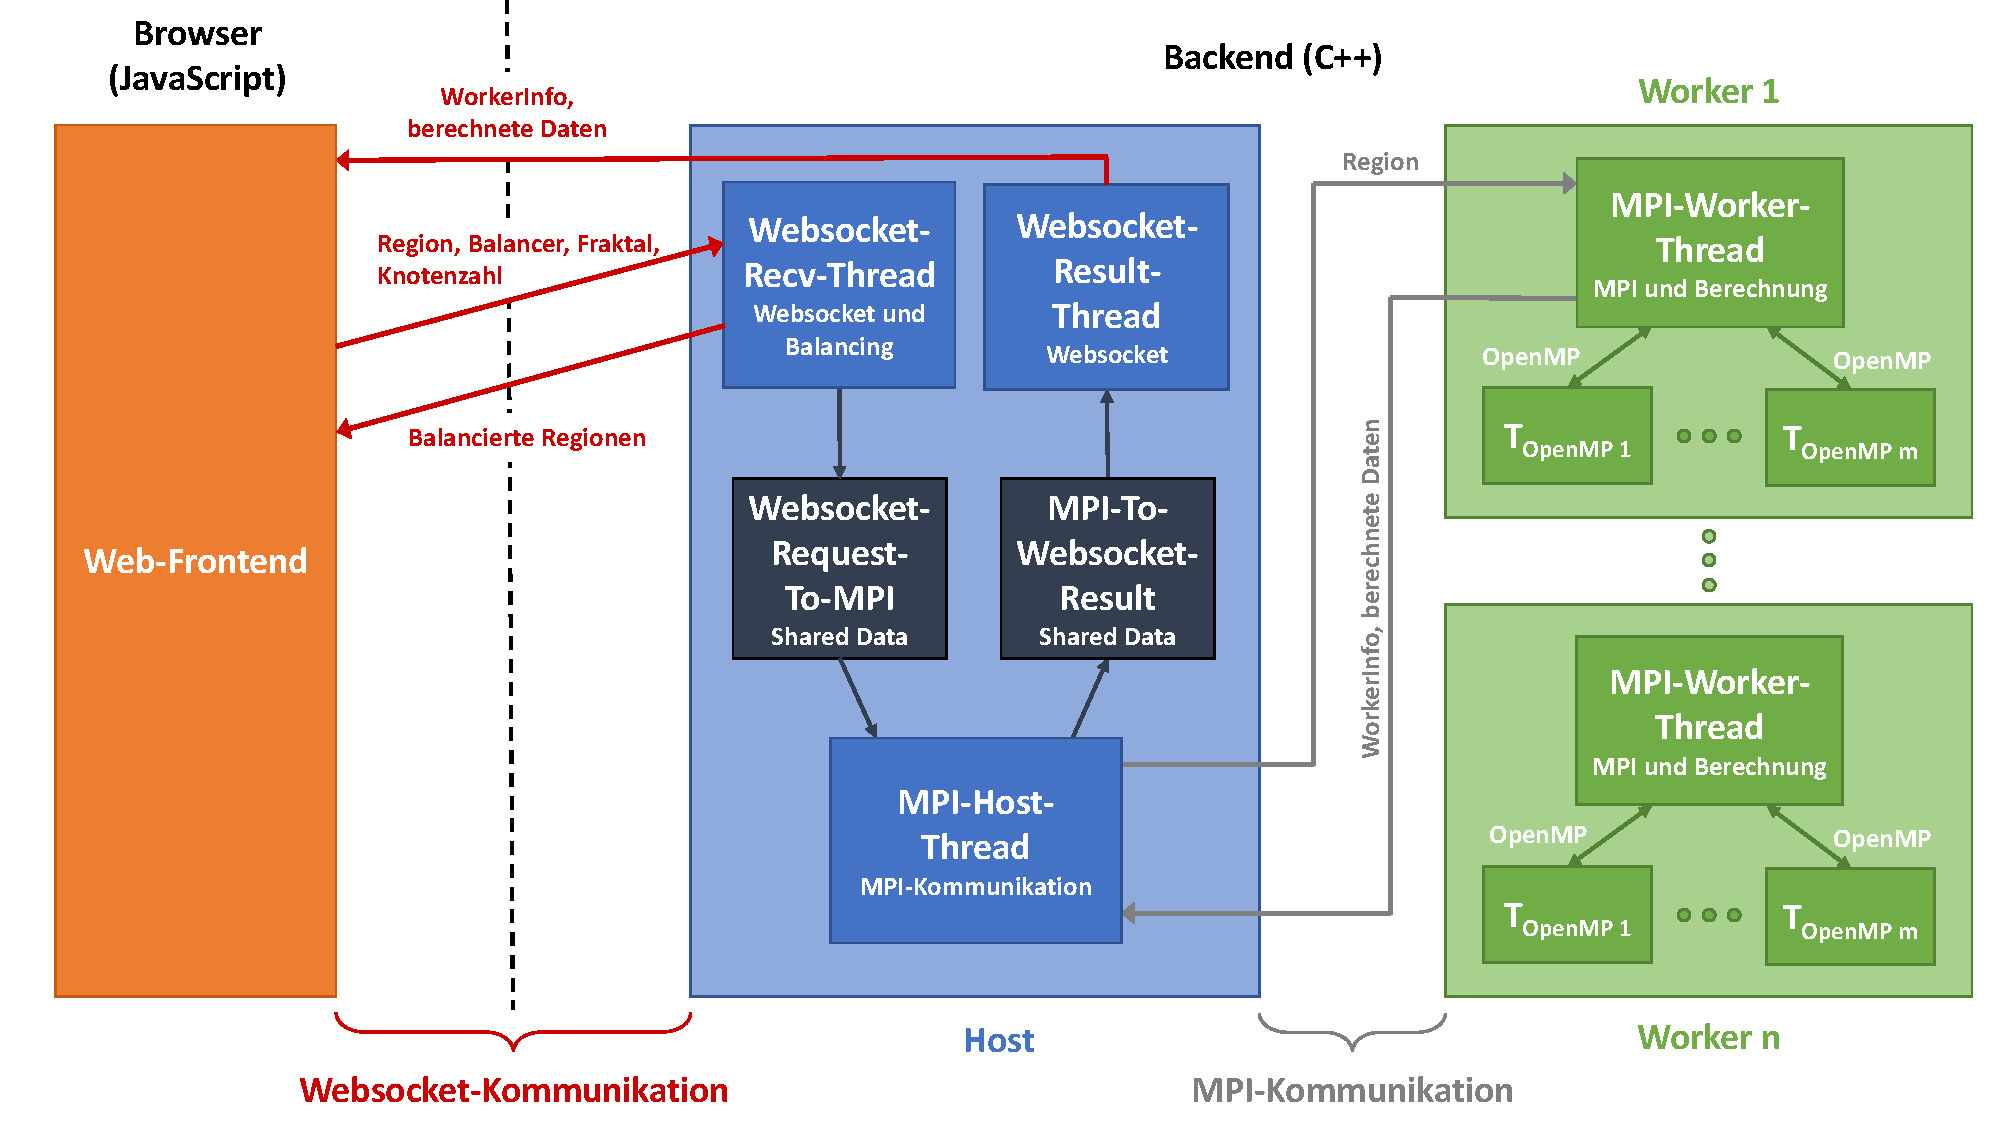
\includegraphics[width=0.98\linewidth]{img/Implementierung/ArchitekturAusfuehrlich.pdf}
	\caption{Detaillierte Architekturübersicht}
	\label{fig:architekturuebersicht_detail}
\end{figure}
Erfolgt eine Nutzereingabe so sendet das Frontend einen entsprechenden Rechenauftrag via Websocket an den Host.
Der Websocket-Recv-Thread des Hosts nimmt den eingehenden Rechenauftrag an, führt das Balancing durch, übermittelt dem Frontend die getätigte Aufteilung und legt diese in der gemeinsamen Datenstruktur Websocket-Request-To-MPI ab.
Der MPI-Host-Thread leitet die in dieser Datenstruktur liegenden Rechenaufträge per MPI an die Worker weiter.
Diese nehmen die zugewiesenen Rechenaufträge entgegen und führen diese ggf. mithilfe von SIMD und / oder OpenMP parallelisiert aus.
Anschließend werden die Rechenergebnisse wieder via MPI an den MPI-Host-Thread übermittelt, welcher diese in der gemeinsamen Datenstruktur MPI-To-Websocket-Result ablegt.
Der Websocket-Result-Thread überträgt die Rechenergebnisse aus der gemeinsamen Datenstruktur per Websocket an das Frontend, wo die Daten verarbeitet und dargestellt werden.



% Welche Lastbalancierungsmechanismen wurden umgesetzt?
\subsection{Lastbalancierung}\label{sec:load_balancing_concepts}
Um die effizienz der parallelen Berechnung der Mandelbrotmenge zu erhöhen, sollte die Rechenlast möglichst gleichmäßig auf die Worker verteilt werden.
Die Aufgabe der Lastbalancierung besteht darin zu einer gegebenen Region und einer Anzahl von Workern eine solche Unterteilung in sogenannte Teilregionen zu finden.
Damit die Unterschiede zwischen guter und schlechter Lastverteilung deutlich werden, stehen in diesem Projekt verschiedene Strategien der Lastbalancierung zur Wahl.
Die Strategien lassen sich zur Laufzeit austauschen, um einen direkten Vergleich zu ermöglichen.

\paragraph{Naive Strategie}
Bei der naiven Strategie wird versucht den einzelnen Workern etwa gleich große Teilregionen zuzuweisen.
Dies geschieht allerdings ohne Beachtung der eventuell unterschiedlichen Rechenzeiten innerhalb der Teilregionen.
Es kann bei Verwendung dieser Stratgegie also durchaus passieren, dass ein Worker noch rechnet, während alle anderen bereits fertig sind.

\paragraph{Strategie mit Vorhersage}
Bei dieser Strategie basiert die Aufteilung der Region auf einer Vorhersage über die Rechenzeit.
Die Teilregionen werden so gewählt, dass sie, entsprechend der Vorhersage, etwa einen ähnlichen Rechenaufwand haben.
Die optimale Rechenlast für einen Worker berechnet sich also durch:

\begin{equation}\label{equ:desiredN}
	\frac{Gesamtrechenlast}{AnzahlWorker}
\end{equation}

Wenn die Vorhersage hinreichend exakt ist, kann dieser Wert gut angenähert werden.
Dadurch wird die Last gleichmäßiger auf die Worker verteilt als bei der naiven Strategie.

\paragraph*{}\label{par:load_balancing_prediction}
Die Zugehörigkeit eines Punktes zur Mandelbrotmenge wird nach \autoref{equ:mandelbrot} iterativ berechnet.
Deshalb kann die Anzahl der benötigten Iterationen als Abschätzung der Rechenzeit für diesen Punkt verwendet werden.
Zur Anstellung der Vorhersage wird also die angeforderte Region in deutlich geringerer Auflösung berechnet.
Dies ist eine gute Annäherung an die tatsächlich Rechendauer, da benachbarte Punkte meist eine ähnliche Anzahl an Iterationen benötigen.
Einzig am Rand der Mandelbrotmenge kommt es zu Ungenauigkeiten, weil dort Punkte innnerhalb und außerhalb der Menge für die Vorhersage zusammenfallen.
Die Genauigkeit der Vorhersage zu erhöhen bedeutet zusätzlichen Rechenaufwand während der Balancierung.
Dieser sollte in einem sinnvollen Verhältnis zum Aufwand der Berechnung der Region selbst stehen.
Es ist also wichtig eine Balance zwischen Güte und Geschwindigkeit der Vorhersage zu finden.

\paragraph{Implementierungsvarianten}
Sowohl die naive Strategie als auch die Strategie mit Vorhersage lassen sich in zwei Varianten umsetzen.
Man kann hierbei einen ganzheitlichen oder einen rekursiven Ansatz wählen.
Bei ersterem wird die gesamte Region in einem Schritt in die gewünschte Anzahl an Teilregionen geteilt.
Dazu werden Zeilen und Spalten gebildet.
Die Grundidee eines rekursiven Ansatzes ist es das Problem so lange in einfachere Teilprobleme aufzuteilen, bis die Lösung offensichtlich ist (Basisfall).
Hier ist der Basisfall die Aufteilung einer Region auf genau einen Worker.
Um diesen zu erreichen wird die Region solange halbiert, bis genug Teilregionen für jeden Worker entstanden sind.

Wo die Grenzen zwischen den Zeilen und Spalten (nicht-rekursiv) bzw. den Hälften (rekursiv) liegen, wird von der zugrundeliegenden Lastbalancierungsstrategie bestimmt.

% Wie wurde die Parallelisierung mit MPI angegangen?
\subsection{Nachrichtenaustausch}
Um eine zwischen den unabhängigen Systemen eine einheitliche Kommunikation zu ermöglichen,
wurde ein Protokoll spezifiziert um Flächen in der komplexen Ebene und ihre Auflösung eindeutig zu bestimmen.
Der grobe Inhalt und die Richtung der Nachrichten ist \autoref{fig:concept_messages} zu entnehmen,
die exakte Spezifikation in der jeweiligen Sprache ist den angegebenen Dateien zu entnehmen.

% austauschen durch tobis
\begin{figure}
	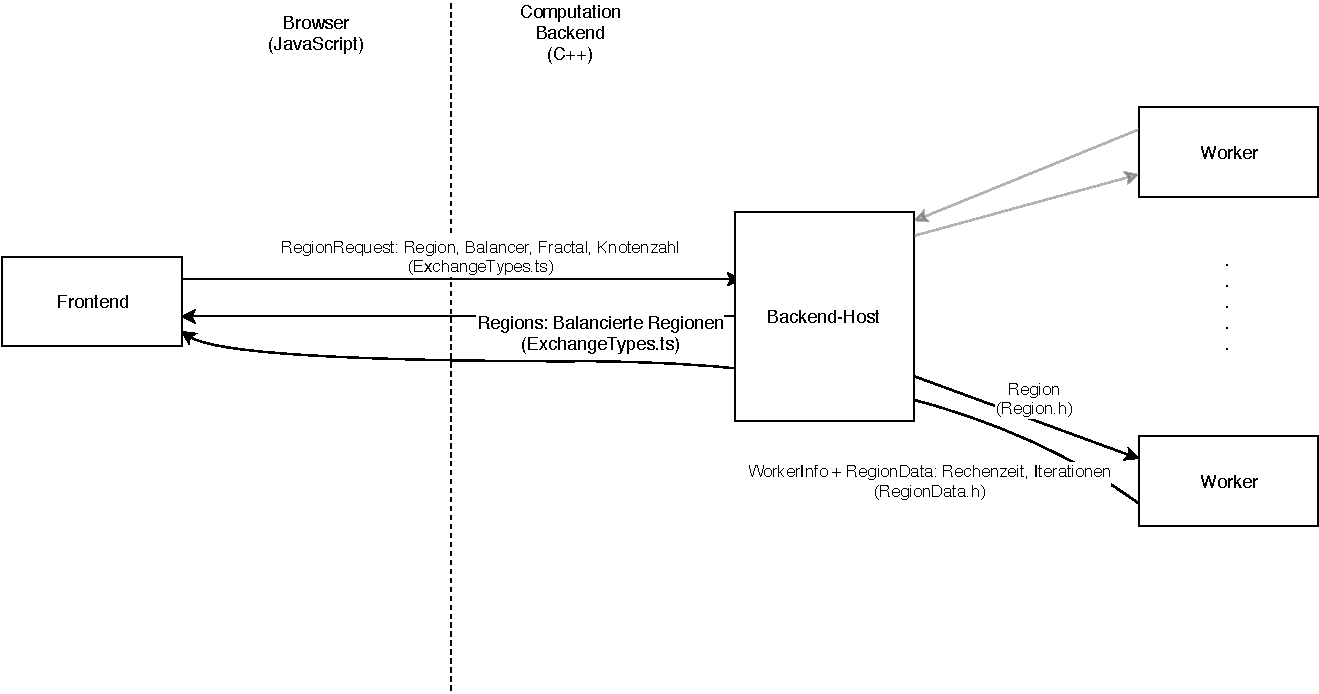
\includegraphics[width=0.9\linewidth]{img/Implementierung/Nachrichtenuebersicht.pdf}
	\caption{Konzept der versendeten Nachrichten. Die genauen Definitionen der Nachrichten sind in den angegeben Dateien nachzusehen.}
	\label{fig:concept_messages}
\end{figure}

% TODO: improve
Ein Beispiel für eine gültige Regionsanfrage ist in \autoref{src:regionRequest.json} zu finden.
Einerseits wird hierbei eine Region in komplexen Koordinaten beschrieben, wobei der obere linke Punkt $(maxImag, minReal)$
und der rechte untere Punkt $(minImag, maxReal)$ in der komplexen Ebene einen zu berechnenden Bereich aufspannen.
Da die reelle Ebene jedoch beliebig genau aufgelöst werden kann, muss zudem noch die Anzahl an Pixeln
pro Seite des Rechteckes definiert werden, \verb|width| und \verb|height|.
Wie in \autoref{fig:concept_coordinates} zu sehen, ist zudem der horizontale Offset und vertikale Offset
die linke obere Koordinate der Region bezüglich der gesamten sichtbaren Anfrage in Pixeln (diese Werte
gewinnen in den Regionsaufteilungen an Bedeutung).
Der Wert \verb|validation| ist technisch gesehen nicht mehr notwendig, wird aber mit dem Zoom-wert der Leafletkarte gefüllt
um zu vermeiden dass Regionsdaten von zuvor berechneten Regionen falsch verwendet werden.

\begin{figure}
	\centering
	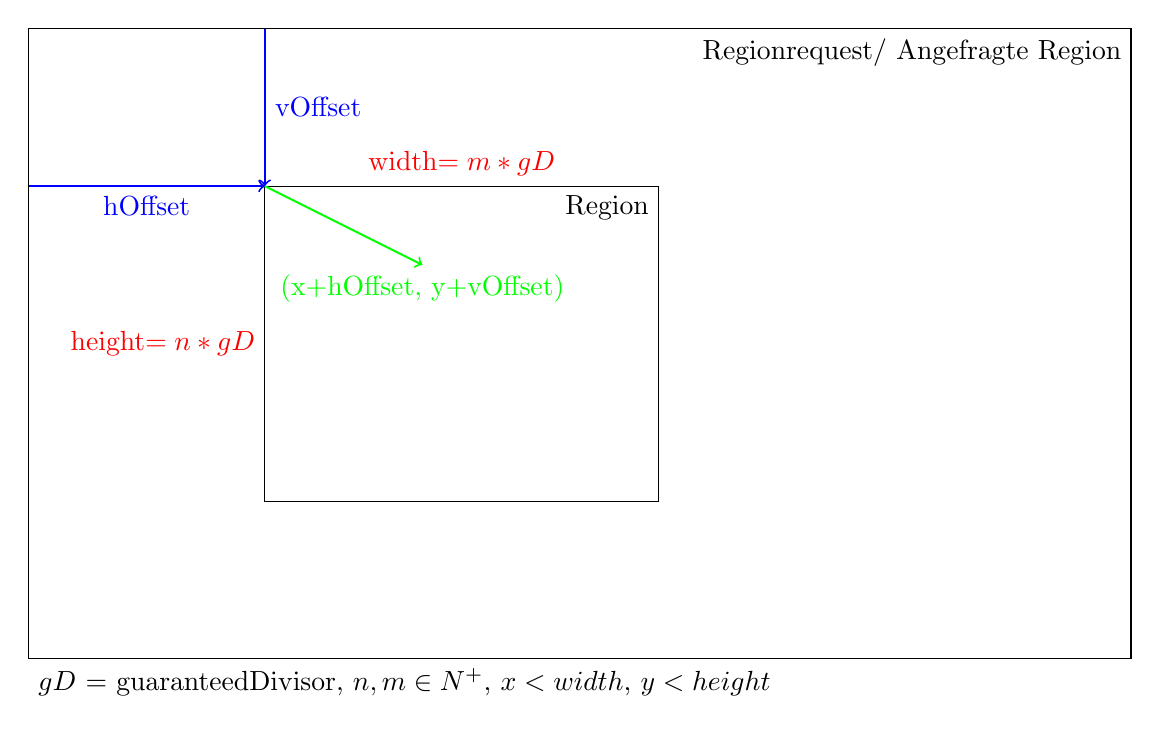
\begin{tikzpicture}[scale=1]
		% Superregion
		\draw (0,0) rectangle (14,8) node[below left] {Regionrequest/ Angefragte Region};
		% subregion
		\draw (3,2) rectangle (8,6) node[below left] {Region};
		% width height
		\draw (3,6) -- node[above, red] {width$=m*gD$} (8,6);
		\draw (3,6) -- node[left, red] {height$=n*gD$} (3,2);
		% vOffset/hOffset
		\draw[blue, ->, line width=0.7pt] (3,8) -- (3,6) node[midway, anchor=west] {vOffset};
		\draw[blue, ->, line width=0.7pt] (0,6) -- (3,6) node[midway, anchor=north] {hOffset};
		% x/y
		\draw[green, ->, line width=0.7pt] (3,6) -- (5,5) node[below] {(x+hOffset, y+vOffset)};
		\draw (0, 0) node[below right] {$gD$ = guaranteedDivisor, $n,m \in \mathbb{N}^{+}$, $x < width$, $y < height$};
	\end{tikzpicture}
	\caption{Konzept der Kooridinaten in den Regionsobjekten. Alle Koordinaten beziehen sich auf die Darstellungsebene und sind daher in Pixeln.}
	\label{fig:concept_coordinates}
\end{figure}

In zurückkehrenden \verb|RegionData|-Nachrichten sind Arrays der berechneten Iterationszahlen eingebunden.
Dabei wird der Punkt (x, y) in der gesendeten Region (Punkt (x+hOffset, y+vOffset) in der angefragten Region)
im Datenarray an Index $i = x + y * width$ gespeichert.

% 1 Seite

% Wie wurde die Parallelisierung mit OpenMP angegangen?
\subsection{Parallelisierung}